\documentclass{article}
\usepackage{amsmath}
\usepackage{graphicx}
\usepackage{algorithm}
\usepackage{algpseudocode}
\usepackage{hyperref}

\title{Real Time traffic Navigation System}
\author{
Ayush Sonika (2023csb1107) \\
Sumit Sharma (2023csb1165) \\
Brajesh Khokad (2023csb1111) \\
Instructor: Dr. Anil Shukla \\
Teaching Assistant: Mr. Deepu Yadav
}
\date{October 1, 2024}

\begin{document}

\maketitle

\begin{abstract}
This project focuses on designing the real time traffic navigation system which contains a graph with nodes as the cities and weights of their edges determine the distance / time required between both the places, this system also uses an AVL tree for efficiently managing and updating traffic data across road segments and  Dijkstra's algorithm for calculating the shortest path in terms of travel time. unlike other traditional algorithm our  system integrates traffic levels as weights to dynamically adjust routes based on real-time congestion data. This system also provide the high traffic situation and also provide a the path that will used in minimum path

\end{abstract}

\section{Introduction}
This document describes the structure and functionality of a traffic-aware pathfinding system developed to address navigation in highly congested areas. Our approach integrates an AVL tree to store and retrieve traffic congestion data efficiently, allowing for rapid updates and access.

The primary components include a graph-based representation of cities and roads, where edges represent road segments with associated weights (distances / time). Traffic congestion data dynamically updates the effective weight of edges, allowing Dijkstra's algorithm to calculate paths optimized for current traffic conditions.

\section{Equations}
Traffic conditions affect travel time by increasing edge weights, which represent road segments in the graph. The total travel time \( T_{total} \) for a path from source \( S \) to destination \( D \) is formulated as:

\[
T_{total} = \sum_{i=1}^{n} \left( d_i + c_i \right)
\]

where:
\begin{itemize}
    \item \( d_i \): distance of segment \( i \),
    \item \( c_i \): congestion cost for segment \( i \).
\end{itemize}

Dijkstra's algorithm is used to minimize \( T_{total} \) by choosing the path with the lowest  weight, adjusted for congestion.

\section{System Components}

\subsection{Graph Representation}
The road network is represented by a graph \( G(V, E) \), where \( V \) is the set of vertices (cities) and \( E \) is the set of edges (road segments). Each edge \( e_{uv} \) between vertices \( u \) and \( v \) has a weight \( w_{uv} \), representing travel distance / total time . Traffic congestion data is stored separately between one place to another and dynamically updates the effective weight.

\subsection{AVL Tree for Traffic Data}
The AVL tree is used to store and retrieve traffic congestion data efficiently, with each node representing a unique road segment. The AVL tree nodes contain:
\begin{itemize}
    \item \textbf{key}: unique identifier for each road segment (edge),
    \item \textbf{traffic}: congestion level, classified as low, moderate, high, or very high.


\end{itemize}

\subsection{Tables}
\begin{table}[h!]
    \centering
    \begin{tabular}{|c|c|}
        \hline
        Traffic Level & Congestion Impact \\
        \hline
        Low & +2 km \\
        Moderate & +4 km \\
        High & +6 km \\
        Very High & +8 km \\
        \hline
    \end{tabular}
    \caption{Traffic congestion levels and their impact.}
\end{table}




\begin{figure}[H]
\centering
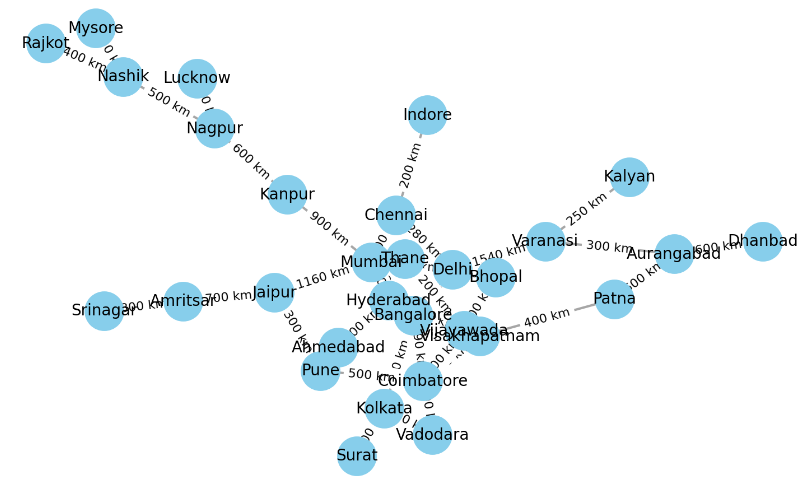
\includegraphics[scale=0.75]{road_network.png}
 \caption{Graph representation with cities as nodes and road segments as edges.}
\end{figure}

\subsection{Algorithms}
\begin{algorithm}
\caption{Traffic-Aware Dijkstra’s Algorithm}
\begin{algorithmic}[1]
    \State Initialize distances from the source to all cities as infinity.
    \State Set the source city's distance to 0 and add it to the priority queue.
    \While{the queue is not empty}
        \State Extract the city \( u \) with the smallest distance.
        \For{each adjacent city \( v \) of \( u \)}
            \State Retrieve traffic congestion \( c \) for the edge \( (u, v) \) from the AVL tree.
            \If{\( \text{dist}[u] + w_{uv} + c < \text{dist}[v] \)}
                \State Update \( \text{dist}[v] \).
                \State Set \( \text{parent}[v] = u \) to reconstruct the path.
            \EndIf
        \EndFor
    \EndWhile
    \State Construct the path from source to destination using parent pointers.
\end{algorithmic}
\end{algorithm}

\section{Results}
Testing was conducted on a garph of 30 cities with dynamically changing traffic congestion data. The AVL tree used to do  efficient updates, while Dijkstra's algorithm provided optimal routes based on the latest traffic conditions. The system detected and avoided highly congested routes, demonstrating potential for real-world applications.

\section{Conclusion}
This project successfully integrates AVL trees with graph-based pathfinding to create a system that dynamically adjusts for traffic congestion. Future enhancements may include incorporating machine learning to predict congestion patterns and refine route efficiency.

\begin{thebibliography}{9}
\bibitem{dijkstra1959}
E.W. Dijkstra, “A Note on Two Problems in Connexion with Graphs,” \textit{Numerische Mathematik}, 1959.
\bibitem{avl1962}
J. Adelson-Velsky and E.M. Landis, “An Algorithm for the Organization of Information,” \textit{Soviet Math. Dokl.}, 1962.
\bibitem{Traffic Management System}
Papageorgiou, A., and W. K. K. Van Zuylen. "Dynamic Traffic Management Systems."
\end{thebibliography}

\end{document}

